\chapter{Úvod}


\chapter{Java Virtual Machine}
Program napsaný v Javě běží typicky v některé z implementací \zkratka{JVM}. \zkratka{JVM} je program, který slouží jako běhové prostředí pro uživatelský kód -- vykonává jeho instrukce a slouží tak jako prostředník mezi ním a operačním systémem (respektive jako interpret jeho kódu, který následně překládá do jiného jazyka, typicky strojového kódu dané architektury či platformy).

Některé implementace \zkratka{JVM} umožňují přímý překlad do strojového kódu bez potřeby interpretace, např. GraalVM \cite{graalvm}. V takovém případě hovoříme o tzv. \zkratka{AOT} přístupu, místo \zkratka{JIT} postupu implementovaného v moderních verzích častěji používaných \zkratka{JVM}, např. HotSpot od společnosti Oracle [TODO zdroj, že HS používá JIT].

\section{Java Bytecode}
Java využívá dvoufázový překlad, tj. samotný zdrojový kód vytvořený programátorem je nejprve přeložen do \textit{bytecodu} (či česky bytekód). Bytecode je (či by měl být) platformě nezávislý soubor instrukcí, který následně \zkratka{JVM} vykoná v prostředí architektury a platformy, na které je spuštěn. To znamená, že zdrojový kód v jazyce Java (či kompatibilních jazycíc využívajících stejné prostředí, např. Kotlin), uložený typicky v souboru \texttt{.java}, je přeložen do bytecodu -- typicky s typu \texttt{.class}. Takové soubory je následně, obecně vzato, možné přenést na jinou platformu či architekturu a jestliže se zde nachází kompatibilní \zkratka{JVM}, je možné jej bez úpravy na daném systému vykonat a tedy program spustit. Bytecode se může přenášet formou klasických jednotlivých souborů \texttt{.class} či v zabalené formě, tj. archiv typu \texttt{.jar} (což je de facto pouze zip archiv s předem danou strukturou a volitelně přidanými informacemi -- manifestem, metadaty, podpůrnými soubory (\textit{resources})).

\chapter{Správa a struktura Java paměti}
Při vytváření programu má programátor na výběr ze dvou způsobů správy paměti -- spravované automaticky (typicky mechanismem typu \zkratka{GC} apod.) či manuálně, případně kombinací těchto přístupů. Ne každý jazyk nabízí oba -- typicky je k dispozici pouze jeden z přístupů, často je správa GC vynucena. Vzhledem k tomu, že majorita nejpopulárnějších programovacích jazyků za poslední roky se řadí mezi vysokoúrovňové, na toto vynucení \zkratka{GC} narazíme u většiny z nich, včetně Javy. Výjimkou jsou populární nízkoúrovňovější jazyky typu C a C++ \cite{stackoverflowinsights}\cite{tiobeindex}.

Paměťovému modelu v Javě se věnuje \textit{JSR-133}, nicméně přesně nespecifikuje konkrétní rozdělení paměti a způsob jejího přidělování a uvolňování. Následný popis se tedy věnuje implementaci od společnosti Oracle – HotSpot. Zde je paměť rozdělena na 2 logické celky – \textit{young generation space} a \textit{old generation space}. Tato paměť, nazývaná \textit{heap} (halda), je rozdělena pouze v rámci JVM a následně je mapována na skutečnou fyzickou paměť \cite{jsr133}.

Young generation space, tedy doslova “prostor mladé generace”, je dále rozdělen na \textit{eden space} a prostory \textit{S0} a \textit{S1}. Eden space slouží k vytváření nových instancí objektů, je zde tedy vyhrazena část paměti nově vytvořenému objektu. Pokud v tomto prostoru není volno, proběhne uvolnění paměti (viz dále) přesunutím některých objektů do S0. Každý takový objekt obsahuje informaci o tom, kolik takových uvolnění daný objekt \uv{přežil}.

Po určitém počtu takových přežití (či jinak také povýšení) je objekt přenesen do objektů staré generace, konkrétně \textit{Tenured space}.

Toto rozdělení objektů do jednotlivých prostorů se jeví jako zbytečná komplikace, má však řadu výhod. První z nich je rychlost – nejvíce operací uvolnění je prováděno právě nad eden spacem, který je z prostorů nejmenší. Dále jsou tak objekty rozdělovány do skupin s podobnou charakteristikou (podobný věk, podobný počet a styl referencí apod.), na kterými je poté možné spustit rozdílné, pro dané skupiny specifické algoritmy pro jejich uvolnění.

\section{Garbage collector}
\zkratka{GC} je nástroj, který odděluje jazyky s automatickou a manuální správou paměti – stará se o její přidělování, kontrolu a následné uvolnění, ať už pokud je jí málo a je zapotřebí jinde, v pravidelných intervalech nebo při jiných událostech. \zkratka{GC} je obecný termín, tj. neodkazuje na žádnou konkrétní implementaci a způsob chování. Často je v rámci jednoho jazyka (respektive běhového prostředí) zároveň implementováno hned několik algoritmů \zkratka{GC} a dle okolností je vybrán ten nejefektivnější a v danou chvíli nejvhodnější z nich. Některé algoritmy tak mohou běžet velmi rychle bez minimálního zásahu do běhu programu, zatímco jiné vyžadují pro svůj běh o něco delší čas. Často tak je nutné všechen běh kódu pozastavit; v takových případech toto spuštění \zkratka{GC} nazýváme \textit{stop-the-world} kolekcí (\uv{zastavení světa}, běhu). Pro program je toto zastavení transparentní.

TODO popis různých implementací GC v Javě?

\section{Heap Dump}
\textit{Heap dump} je textová nebo binární reprezentace paměti, kterou je možné uložit na disk a zachycuje aktuální stav aplikace. Při vytváření je činnost aplikace pozastavena. Dump je možné následně analyzovat a dále zpracovávat, je tak možné prozkoumat vnitřní stav aplikace v určitém bodě a např. řešit příčiny neočekávaného chování. 

\subsection{Vytvoření dumpu}
Prostředků k vytvoření dumpu je několik. Při správném nastavení (pomocí parametru \texttt{HeapDumpOnOutOfMemoryError}) k němu dojde při nedostatku paměti zcela automaticky. Mezi manuální způsoby vytvoření patří primárně nástroj \textit{JMAP}, který je publikován spolu se standardní distribucí Oracle JVM. Při použití tohoto nástroje je nutné naprosto přesně dodržet číslo verze JMAP a JRE, pod kterým cílová aplikace běží – dumpování rozdílných verzí není podporováno, je nutné dodržet rovnost verzí (major, minor i update).

Mezi další způsoby vytvoření dumpu patří různé nástroje, debuggery a profilery typu Eclipse MAT, VisualVM nebo Java Mission Control (viz dále). Výhodou těchto nástrojů je, že dokáží zvládnout vytváření dumpu i napříč verzemi a dokonce implementacemi (z Oracle JDK na OpenJDK apod.)

Další možnost je využít některou z knihovních funkcí a vytvářet tak dump programově. Zde je možné využít např. MBeans. Nízkoúrovňovou možností je poté například použití Unixového nástroje \textit{gcore}, respektive \textit{GDB}, který se postará o vytvoření dumpu paměti procesu (pod daným \zkratka{PID}), tzv. \textit{core dump}. Z něj lze memory dump vyextrahovat. Pokročilejší nástroje typu VisualVM umí pracovat i napřímo s core dumpem.

\subsubsection{Vztah dumpu vůči paměti procesu}
Heap Dump přímo odpovídá části paměťového prostoru procesu, resp. heapu. Je tedy přímým otiskem části fyzické paměti tak, jak je uložena, v určitém časovém okamžiku. Toto je možné si experimentálně ověřit -- jak bylo zmíněno výše, z otisku fyzické paměti je možné heap dump získat. Je tedy evidentní, že při jeho vytvoření některým z výše uvedených způsobů nedochází k žádným úpravám a snímek je vytvořen \uv{tak jak je}. 

\begin{figure}[h]
	\centering
	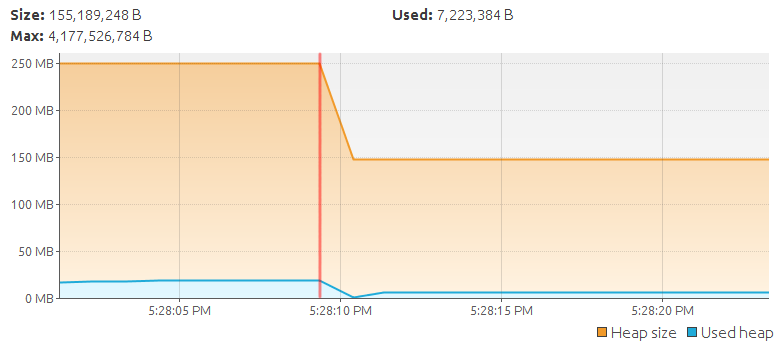
\includegraphics[scale=0.5]{obrazky/heapdump-performed.png}
	\caption{Využití paměti a provedení garbage kolekce před vytvořením dumpu (červeně).}
	\label{obr1}
\end{figure}

\section{Zpracování dumpu}
Při zpracování dumpu je nutné zohlednit fakt, že je vyexportovaný kompletní paměťový prostor [TODO zdroj] a nachází se zde tedy i data objektů, které nás nutně nemusí zajímat – typicky knihovny nebo objekty Javy. Toto je možné zohlednit a filtrovat na základě jmenného prostoru (namespace), do kterého objekt patří.

Pro práci nad heapem  (typicky ve formátu HPROF) je možné využít některou z implementací dotazovacího jazyku OQL (Object Query Language).

\chapter{Analýza paměti}

\chapter{Analýza zbytečného čerpání paměti}

\chapter{Existující nástroje pro analýzu heapu}

\section{Eclipse MAT}
IBM Eclipse Memory Analyser Tooling je open source nástroj pro analýzu Java paměti. Po spuštění umožňuje otevřít již vygenerovaný dump Java heapu, umí jej ale i vytvořit. V rámci analýzy nabízí 2 konkrétní volby – analýzu memory leaků a memory bloatu – tj. neefektivního využití paměti a zbytečného plýtvání. 

MAT se analýzou memory bloatu přibližuje zamýšlenému výsledku této práce, bohužel ale nenabízí kompletní funkcionalitu v této oblasti. Omezuje se pouze na efektivní práci s řetězci (kterou už obsahuje Java, respektive JVM v základu, viz TODO) a dalšími základnímu typy, např. Map. Cílem práce je ale zpracování všech možných objektů, tato funkcionalita by se tak dala případně rozšířit.

Nástroj je založený na platformě Eclipse RCP (Rich Client Platform), respektive OSGi. Díky tomu je poměrně snadno rozšiřitelný, což je ale vyváženo velkým rozsahem aplikace, který vývoj a rozšíření naopak lehce komplikuje. Buildovacím nástrojem je zde Maven.

\section{VisualVM}
Open source profiler pro Java platformu. Patří mezi nejpoužívanější profilery, respektive nástroje pro analýzu výkonu v Javě.

Po spuštění nabízí klasické funkce typické pro profilery, tj. využití paměti, zatížení CPU, počet objektů a vláken a podobné statistiky. Kromě toho obsahuje celou řadu dalších funkcí, jako provedení garbage kolekce (její vyžádání, explicitně vyvolání GC není možné) nebo vytvoření heap dumpu.

Požadovanou funkcionalitu VisualVM v zásadě neposkytuje, umožňuje pouze k nahlédnutí tabulku s informacemi – kolik bylo vytvořeno instancí jaké třídy, respektive jimi okupovanou paměť. V programu využít podporu pro OQL syntaxi, což je možné využít, nicméně tento přístup nelze považovat za dostačující.

Pro build je využíván nástroj Ant a v současné době je vyžadována Java verze 7 a vyšší.

\section{Java Mission Control}
Nástroj poskytovaný přímo spolu s distribucí Oracle JVM od verze 7 (konkrétně 7 Update 40 – 7u40), což je jeho výhodou. Mezi jeho možnosti patří např. využití paměti jednotlivými součástmi Java paměti (TODO: popsat spaces – eden space atd) a také umožňuje zobrazit jednotlivé instance objektů, nicméně neumožňuje jejich další analýzu.

\section{JProfiler}
Komerční profiler, přesto velice používaný. Standardní licence stojí v době psaní 409 euro, akademická potom 179 euro. Je možné zažádat o licenci pro open source produkty, nicméně ta je podmíněna již vydanou verzí a existující webovou stránkou, což činí jakékoliv použití tohoto profileru v rámci práce nepraktickým. Profiler je používán především v komerční sféře, díky svým možnostem a dle výše uvedeného testu i nejvyšší úspěšností v odhalování bugů.

\chapter{Možnosti analýzy}
Rovnost dvou či více objektů se dá definovat a zjišťovat různými způsoby. Je ale nutné si uvědomit, že v nejhorším případě, tj. pokud chceme najít všechny nadbytečné kopie každého objektu, je složitost této operace při nejmenším $O(n^n)$. Bylo by tedy vhodné se zamyslet, zda neexistuje způsob, jak počet porovnání snížit, případně navrhnout jednoduchou heuristiku, která by dokázala rychle ohodnotit, zda má vůbec smysl pokračovat v podrobnějším porovnání. V následujících případech tedy uvažujme objekty $A$, $B$, jejich třídy $C_A$ a $C_B$ a proměnné obou instancí $F_A^0..F_A^n$, respektive $F_B^0..F_B^n$.

První nápovědou samozřejmě může být porovnání tříd obou objektů -- $C_A$ a $C_B$. Pokud platí $C_A = C_B$, zřejmě má smysl se porovnáváním dále zabývat. V případě jejich nerovnosti není ale možné další porovnání zavrhnout, porovnat je nutné (či možné) i jejich rodiče. Definujeme-li tedy funkci pro zjištění přímého rodiče $P(C)$, potom rovnost objektů lze vyjádřit jako
    $$ E(C_A, C_B) \Leftrightarrow C_A = C_B \vee E(P(C_A), C_B) \vee E(C_A, P(C_B)).$$    
Samozřejmě je nutné definovat i zastavovací podmínku, v případě Javy by tedy jeden z parametrů nesměl být třída typu \textit{Object}. Formálně je tedy možné tuto rovnost definovat jako
	$$ E(C_A, C_B) = P_c(C_A) \cap P_c(C_B) \notin \emptyset,$$
kde $P_c(C)$ je množina třídy samotné a všech jejich rodičů bez “univerzálního předka” všech tříd, v tomto případě \textit{Object}:
	$$ P_c(C) = \{C, P(C), P(P(C)), \dots, Object\} \setminus Object. $$
Nejjednodušší cestou je prosté porovnání hodnot jednotlivých


\chapter{Analýza a implementace}
